\documentclass[acmtog, authorversion]{acmart}

\usepackage{booktabs} % For formal tables

% TOG prefers author-name bib system with square brackets
\citestyle{acmauthoryear}
\setcitestyle{square}

\usepackage[ruled]{algorithm2e} % For algorithms
\usepackage{enumitem}
\usepackage{siunitx}

\renewcommand{\algorithmcfname}{ALGORITHM}
\SetAlFnt{\small}
\SetAlCapFnt{\small}
\SetAlCapNameFnt{\small}
\SetAlCapHSkip{0pt}
\IncMargin{-\parindent}

% Metadata Information
\acmJournal{TOG}
\acmVolume{X}
\acmNumber{X}
\acmArticle{XX}
\acmYear{2019}
\acmMonth{4}

% Copyright
%\setcopyright{acmcopyright}x
%\setcopyright{acmlicensed}
%\setcopyright{rightsretained}
%\setcopyright{usgov}
\setcopyright{usgovmixed}
%\setcopyright{cagov}
%\setcopyright{cagovmixed}

% DOI
\acmDOI{0000001.0000001_2}

% Paper history
\received{April 2019}
\received{Month 2019}
\received[final version]{Month 2019}
\received[accepted]{Month 2019}


\newcommand{\jhnote}[1]{{\textcolor{blue}{FH: #1}}}
\newcommand{\scnote}[1]{{\textcolor{red}{SC: #1}}}
\newcommand{\alnote}[1]{{\textcolor{orange}{JR: #1}}}
\newcommand{\norm}[1]{\lVert #1\rVert}

% Document starts
\begin{document}
% Title portion
\title{A Brief Introduction to GAIL ({\sc Guaranteed Automatic Integration Library}) Version 2.3}

\author{Sou-Cheng T.~Choi}
\orcid{0000-0002-4270-7077}
\affiliation{%
  \institution{Illinois Institute of Technology}
  \streetaddress{10 W 32nd St}
  \city{Chicago}
  \state{IL}
  \postcode{60637}
  \country{USA}}
\email{schoi32@iit.edu} 
\author{Jagadeeswaran Rathinavel}
\orcid{0000-0002-4270-7077}
\affiliation{%
  \institution{Illinois Institute of Technology}
  \streetaddress{10 W 32nd St}
  \city{Chicago}
  \state{IL}
  \postcode{60637}
  \country{USA}}
\email{jrathin1@hawk.iit.edu} 
\author{Xin Tong}
\orcid{0000-0002-4270-7077}
\affiliation{%
  \institution{University of Illinois at Chicago}
  \streetaddress{1200 W Harrison St}
  \city{Chicago}
  \state{IL}
  \postcode{60607}
  \country{USA}}
\email{xtong5@hawk.iit.edu} 
\author{Kan Zhang}
\orcid{0000-0002-4270-7077}
\affiliation{%
  \institution{Illinois Institute of Technology}
  \streetaddress{10 W 32nd St}
  \city{Chicago}
  \state{IL}
  \postcode{60637}
  \country{USA}}
\email{kzhang23@hawk.iit.edu} 
\author{Fred J.~Hickernell}
\orcid{0000-0002-4270-7077}
\affiliation{%
  \institution{Illinois Institute of Technology}
  \streetaddress{10 W 32nd St}
  \city{Chicago}
  \state{IL}
  \postcode{60637}
  \country{USA}}
\email{hickernell@iit.edu} 

\renewcommand\shortauthors{Choi, S.-C. et al}


\begin{abstract}
Function approximation, optimization, and integration over (in)finite
domains are among the most fundamental mathematical problems. They  are
particularly challenging when the functions in consideration fluctuate
wildly in certain parts of the domain or if the domain is high dimensional.
Development of efficient and effective numerical algorithms for
approximating the solutions to these problems that are based on rigorous
mathematical frameworks, (statistical) error bounds, advanced sampling
strategies, and careful complexity analysis remain active research areas. 
The Guaranteed Automatic Integration Library (GAIL) %~\cite{ChoEtal18b} 
is our multi-year research efforts directed towards addressing the
aforementioned overarching theme. Briefly, GAIL is an open-source MATLAB
software package with eight main algorithms based on over ten peer-reviewed
publications, involving more than nine doctoral students and three faculty
members in Illinois Tech as well as their international collaborators.  The
theories behind our algorithms consider functions in cones, rather than
balls, and then proceed to sample data points of a given function in an
adaptive manner, placing more samples in areas where the function changes
faster. Our algorithms are iterative in nature, with errors bounds computed
in each iteration. They are proven to have optimal costs, with monotonic
decreasing error estimates and stop in the first iteration where user-given
tolerance is met.  We consistently employ proven industrial software
development practices for GAIL such as unit and integration tests,
searchable online and offline documentation, version control systems
(GitHub), and agile methodology (using Trello). Our reproducible research
have demonstrated that GAIL could outperform more established algorithms in
various ways.   
\end{abstract} 


%
% The code below should be generated by the tool at
% http://dl.acm.org/ccs.cfm
% Please copy and paste the code instead of the example below.
%
\begin{CCSXML}
<ccs2012>
 <concept>
  <concept_id>10010520.10010553.10010562</concept_id>
  <concept_desc>Computer systems organization~Embedded systems</concept_desc>
  <concept_significance>500</concept_significance>
 </concept>
 <concept>
  <concept_id>10010520.10010575.10010755</concept_id>
  <concept_desc>Computer systems organization~Redundancy</concept_desc>
  <concept_significance>300</concept_significance>
 </concept>
 <concept>
  <concept_id>10010520.10010553.10010554</concept_id>
  <concept_desc>Computer systems organization~Robotics</concept_desc>
  <concept_significance>100</concept_significance>
 </concept>
 <concept>
  <concept_id>10003033.10003083.10003095</concept_id>
  <concept_desc>Networks~Network reliability</concept_desc>
  <concept_significance>100</concept_significance>
 </concept>
</ccs2012>
\end{CCSXML}

\ccsdesc[500]{Computer systems organization~Embedded systems}
\ccsdesc[300]{Computer systems organization~Redundancy}
\ccsdesc{Computer systems organization~Robotics}
\ccsdesc[100]{Networks~Network reliability}

%
% End generated code
%


\keywords{adaptive sampling, function approximation, global optimization, quasi-Monte Carlo}

\maketitle

\section{Introduction} \label{sec:intro}

Numerical algorithms for integration, function approximation and
optimization attempt to provide approximate solutions that differ from the
true solutions by no more than a user-specified error tolerance. The
computational cost is often determined adaptively by the algorithm based on
the function values sampled. While adaptive algorithms are widely used in
practice, most lack guarantees, i.e., conditions on input functions that
ensure the error tolerance is met. The GAIL software library~\cite{ChoEtal18b},
developed by our collaborators and us, is an attempt to provide guaranteed
numerical algorithms with certain well-defined assumptions.

The mathematical problems of concern to us involve an input function $f$
with a domain $\mathcal{D} \subseteq \mathbb{R}^d$ for some $d \in \mathbb{N}$.
Traditional approaches would  consider $f$ to be in some space
$\mathcal{S}$ and derive algorithms that are guaranteed for inputs in a ball, $\{f \in \mathcal{S}: \norm{f} \le \alpha \}$, of radius $\alpha >0$.  GAIL's underlying
theories~\cite{clancy2014cost} are built on the assumption that the input is in a
cone, e.g., $\{f  \in \mathcal{S}:\norm{f} \le \alpha \norm{f}_w \}$ for
some $\alpha >0$ and a weaker norm $\norm{\cdot}_w$ than $\norm{\cdot}$.  Although the GAIL originally emphasized integration problems, its scope has expanded to include function approximation and optimization.

For univariate function approximation on a finite interval $[a,b]$, GAIL
considers the space $\mathcal{S}$ to be the Sobolev space
$\mathcal{W}^{2,\infty}[a,b]$ and constructs an approximation $\hat{f}$ as a linear
splines such that the error estimate $\norm{f - \hat{f}} \le \varepsilon$,
where $\varepsilon>0$ is a given
tolerance~\cite{FunappxFunmin,clancy2014cost}.

For univariate function minimization~\cite{FunappxFunmin}, GAIL builds on
the function approximation approach and bounds segments of $f$  between
sampling points with $\hat{f}$ and a quadratic function fitted to the
neighboring data points, so that we could bound the  error $|x^*-\hat{x}|$,
where $x^* := \argmin_{x \in [a,b]} f(x)$ and $\hat{x}$ is an approximate location of the 
minimum.

Multiple cubatures~\cite{cubBayesLattice,cubSobol,cubLattice,meanMCcubMC}
are available from GAIL for high-dimensional integration, $ \mu = \int_{x
\in [0,1]^d} f(x) \, dx$ with guaranteed accuracy. The adaptive quasi-Monte Carlo algorithms \texttt{cubSobol\_g}
and \texttt{cubLattice\_g} assume that the Fourier coefficients of $f$ decay steadily,
whereas \texttt{cubBayesLattice\_g} considers $f$ to be an instance of a
Gaussian process.

Another key feature to all GAIL algorithms is that the number of samples, $n$, is automatically determined by data-driven approaches. GAIL's
univariate approximation and optimization algorithms place sampling points
at higher density where $f$  changes faster. Hence, they tend to be more
capable of handling functions with spikes efficiently. Error bounds derived
from the cone framework are also computed and used in stopping criteria of
these iterative methods.

We refer readers to the cited references for full details, definitions of
cones, pseudocode,  and proofs of optimal order of costs.
 %in terms of $n$,   $\norm{f}$, and/or $\varepsilon$.
 
% A Theory section should extend, not repeat, the background to the
% article already dealt with in the Introduction and lay the
% foundation for further work.

\section{Overview}
\label{sec: overv}

TBD
 



\section{Algorithms}
\label{sec:algo}

GAIL's latest release, version 2.3, includes the following algorithms:
\begin{enumerate} [label=\Roman*.]

\item Approximation and optimization:

    \begin{enumerate}[label={[\arabic*]}]
    
    \item \texttt{funappx\_g}: One-dimensional function approximation on bounded interval~\cite{FunappxFunmin}
    
    \item \texttt{funmin\_g}: Global minimum value of univariate function on a closed interval~\cite{FunappxFunmin}
    
    \end{enumerate}

\item Integration:

    \begin{enumerate}[label={[\arabic*]}, start=3, resume*]
    
    \item \texttt{integral\_g}: One-dimensional integration on bounded interval~\cite{ChoEtal18b}
    
    \item \texttt{meanMC\_g}: Monte Carlo (MC) method for estimating mean of a random variable~\cite{meanMCcubMC}
    
    \item \texttt{meanMC\_CLT}: MC method with Central Limit Theorem (CLT) confidence intervals for estimating mean of a random variable \cite{ChoEtal18b}
    
    \item \texttt{cubMC\_g}: MC method for  multiple integration \cite{meanMCcubMC}
    
    \item \texttt{cubSobol\_g}: Quasi-Monte Carlo (QMC) method using Sobol' cubature for multiple integration \cite{cubSobol}
    
    \item \texttt{cubLattice\_g}: QMC method using rank-1 lattices cubature for multiple integration \cite{cubLattice}
    
    \item \texttt{cubBayesLattice\_g}: Bayesian cubature method using lattice sampling for multiple integration \cite{cubBayesLattice}
    
    \end{enumerate}
\item Option Pricing:
\begin{enumerate}\setlength\itemsep{1em}
\item \texttt{assetPath}: A class of discretized stochastic processes that model the values of an asset with respect to time \cite{ChoEtal18b}
\item \texttt{optPayoff}: A class of option payoffs based on asset paths \cite{ChoEtal18b}
\item \texttt{optPrice}: A class that computes the price of an option via (quasi-)Monte Carlo methods \cite{ChoEtal18b}
\end{enumerate}

\end{enumerate}


 
\section{Numerical Examples}
\label{sec:ex}

In this section, we showcase GAIL's performance with two examples on
univariate function optimization and cubature.

\begin{example}\label{eg1} We want to find the global minimum of the following functions: 
\begin{align}
    f(x) &= -5 \E^{-100(x-0.15)^2}-\E^{ -80(x-0.65)^2}  \mbox{ for } x \in [0, 1], \label{eq1}
\\  f(x) &= \sin (10 \pi x^4 ) - x  \mbox{ for } x \in [0, 2]. \label{eq2}
\end{align}
In the case of (\ref{eq1}), \texttt{funmin\_g} automatically samples the
function more often in spiky areas and locates the global minimum
accurately. In contrast, MATLAB's
\texttt{fminbnd}~\cite{brent2013algorithms,forsythe1977computer} returns a
local minimum.  That said, we note that \texttt{fminbnd} was designed for
seeking a local minimum. Chebfun~\cite{TrefEtal17a} approximates $f$ with
Chebyshev polynomials and samples $f$ at Chebyshev points. Its \texttt{min} function is 
capable of returning all local minimum that it
could find, out of which we extract the global minimum. Both \texttt{min} and
\texttt{funmin\_g} succeeded in locating the global minimum to required
accuracy, with the former being more efficient with fewer sampling points
and the latter more accurate.


In the case of (\ref{eq2}), we have a function that is increasingly
oscillating as $x$ increases and the true minimum occurs at the right
boundary point. Both \texttt{min} and \texttt{funmin\_g} were able to return  
accurate approximations, but \texttt{fminbnd} once again settled at a local
minimum far away from the global minimum. The total run time of
\texttt{funmin\_g} was substantially less than that of \texttt{min} because it
sought only the global minimum and disregarded the other local minima.

We plot $f(x)$ and the minima returned by \texttt{funmin\_g}, \texttt{min},
and \texttt{fminbnd}  for the two given functions in Figures~\ref{fig1} and
\ref{fig2}. In addition, Table~\ref{tab1} summarizes the solvers'
performance.

\begin{figure} % MATLAB Driver: min_pearc.m
\centering
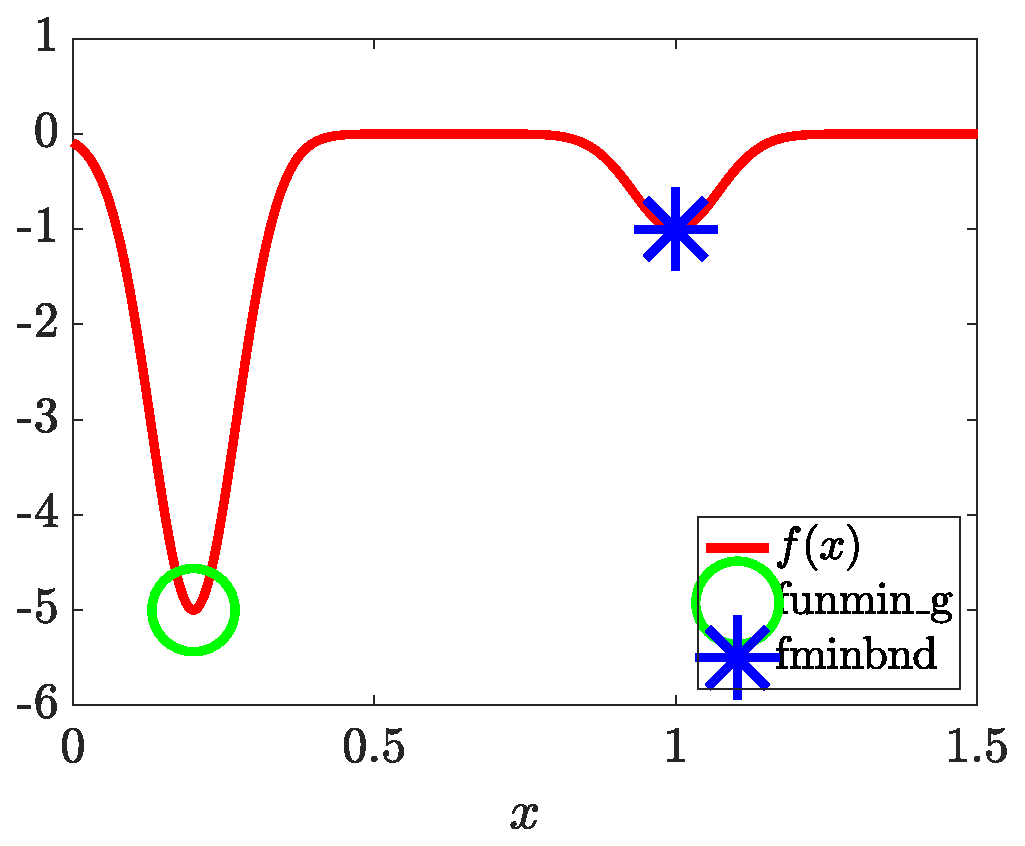
\includegraphics[width = 0.48\textwidth]{humps.eps} 
\caption{We plot the function $f$ in (\ref{eq1}), along with the sampling
points and best estimates of $(x^*, f(x^*)$ from the three solvers,
MATLAB's \texttt{fminbnd}, Chebfun's \texttt{min}, and GAIL's \texttt{funmin\_g}. 
This figure is
reproducible by the MATLAB script, \texttt{min\_pearc.m}, in GAIL.}\label{fig1}
\end{figure}

\begin{figure} % MATLAB Driver: min_pearc.m
\centering
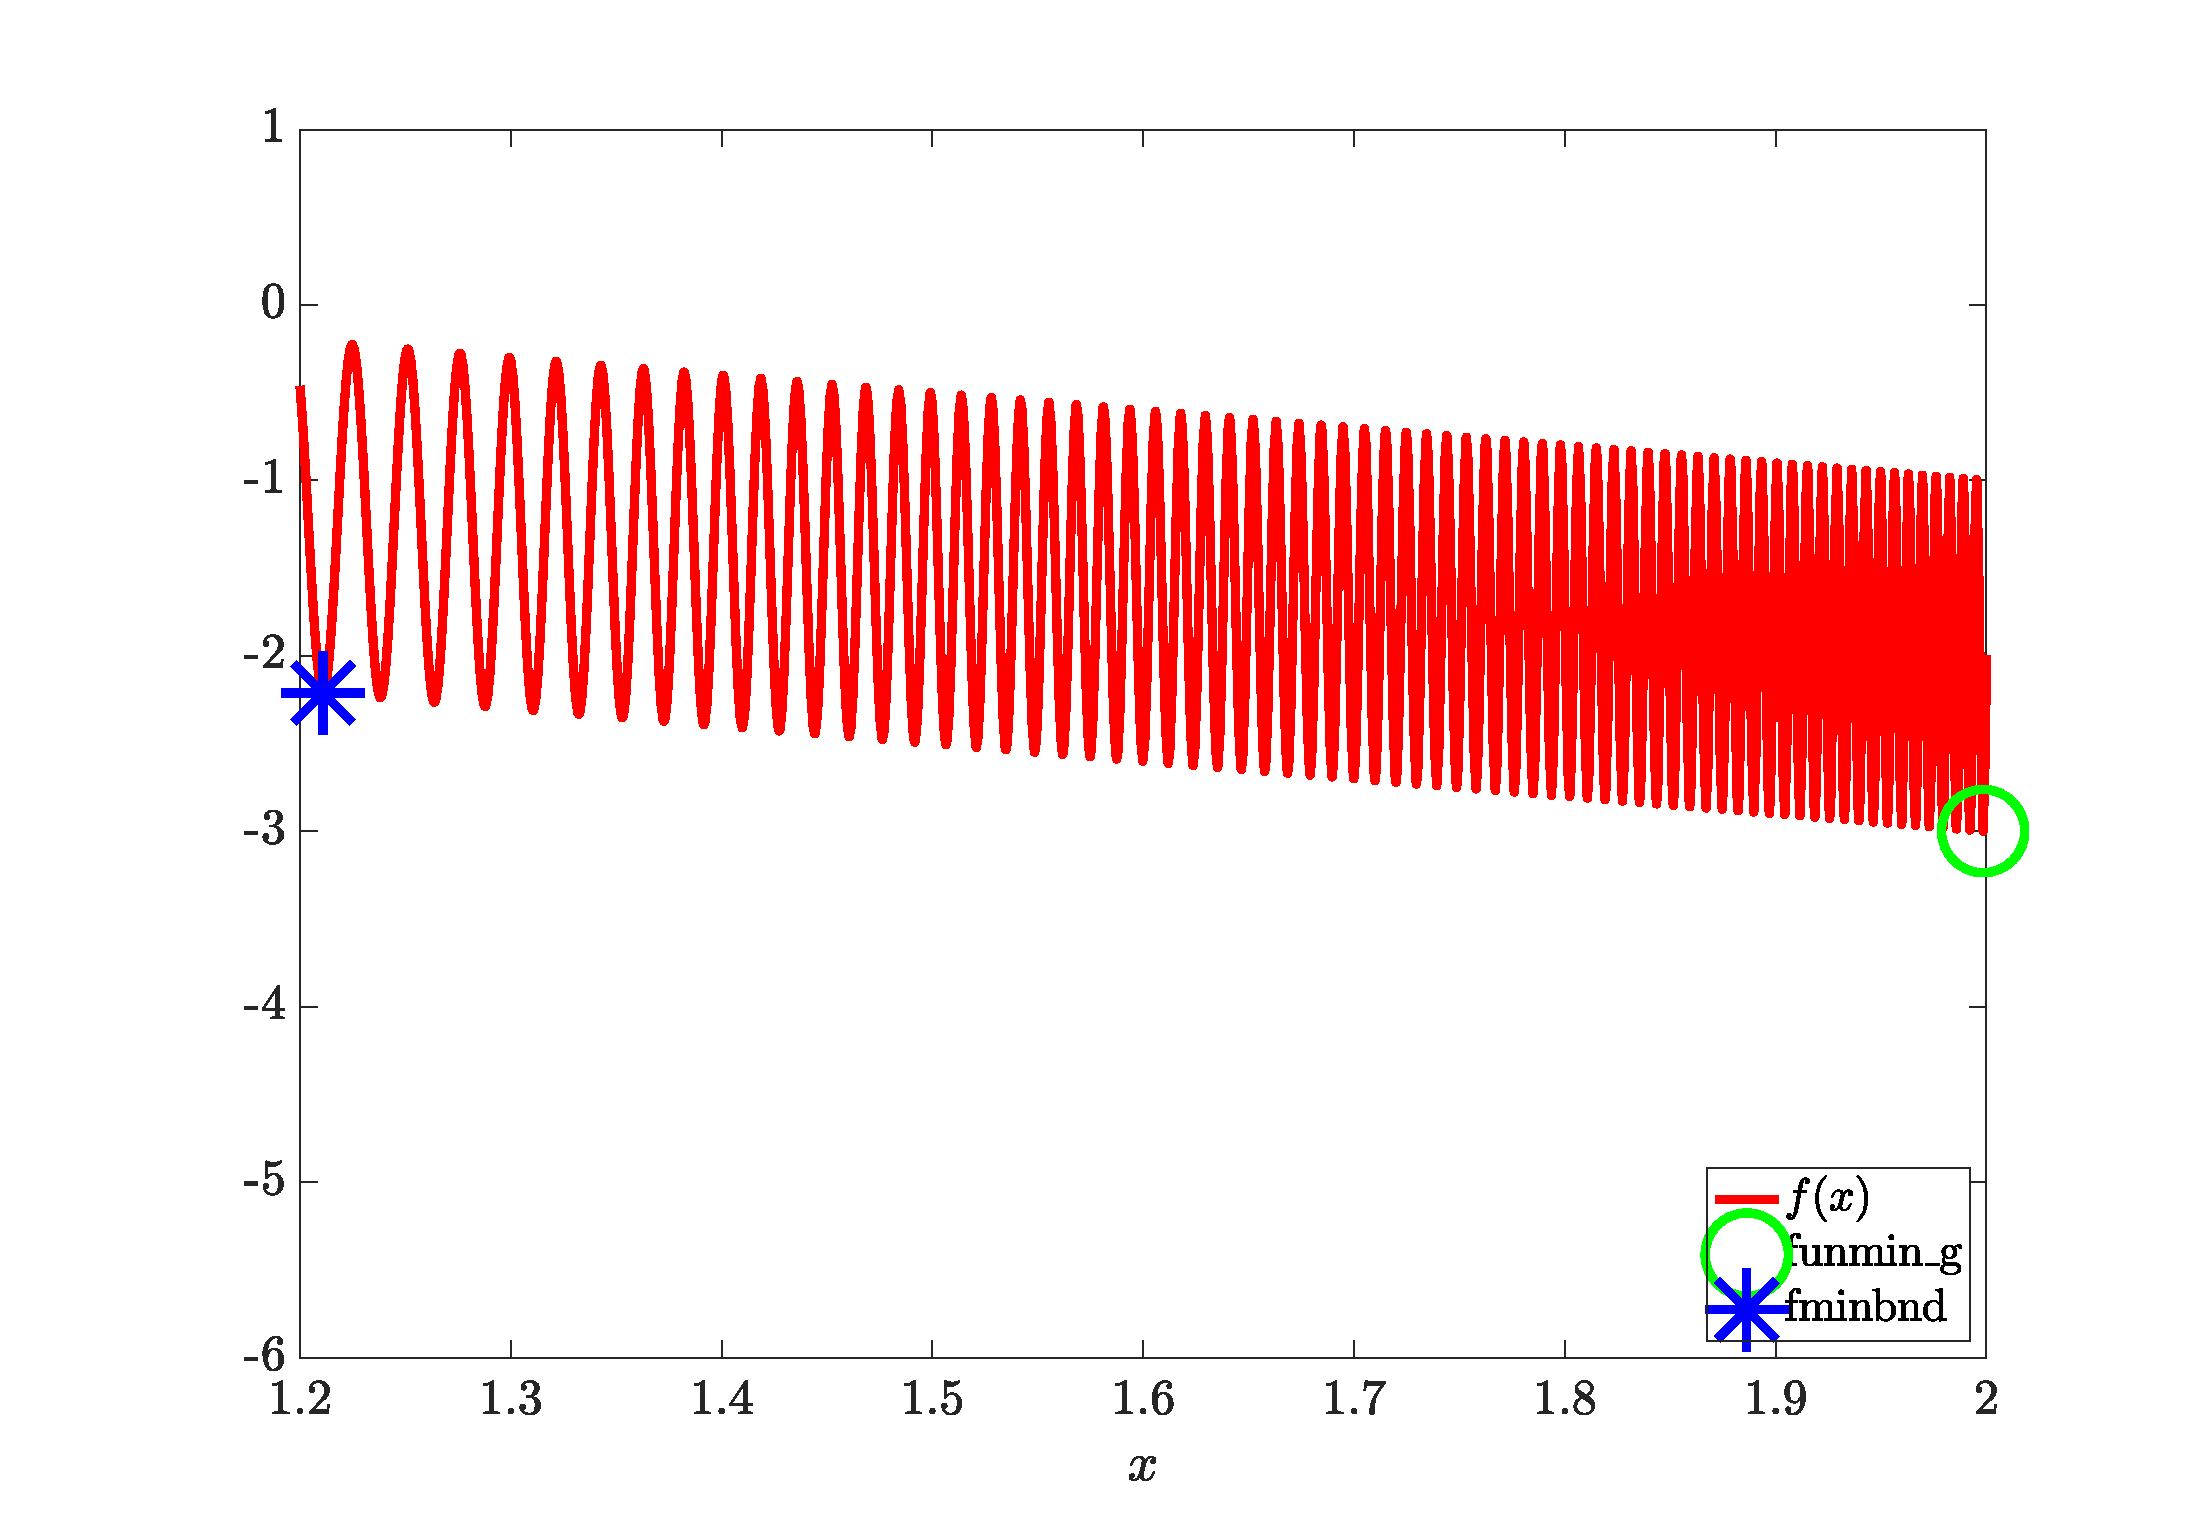
\includegraphics[width = 0.48\textwidth]{sine.eps} 
\caption{
This figure is reproducible by the script, \texttt{min\_pearc.m}, in GAIL.}\label{fig2}
\end{figure}

\begin{table} % MATLAB Driver:  min_pearc.m
\centering
	\caption{Performance of \texttt{funmin\_g}, \texttt{fminbnd}, and
	\texttt{min} with automatic stopping criteria for optimizing
	functions defined in (\ref{eq1}) and (\ref{eq2}). Absolute errors in
	$x$  and $y$ are defined as $|x^* - \hat{x}|$ and $|f(x^* ) -
	f(\hat{x})|$, respectively. These results can be reproduced with script
	\texttt{min\_pearc.m} in GAIL. \label{tab1}}  \vspace{-2ex}
	$
    \begin{array}{l@{\qquad}r@{\quad}r@{\quad}r}
	\input{minPearcOut.txt} 
	\end{array}
	$
\end{table}
\end{example}


\begin{example}\label{eg4}  
In this example, we compare GAIL's Monte Carlo and quasi-Monte Carlo
methods in similar ways as in Section~4 in \cite{hickernellmonte} with the
Keister integrals~\cite{keister1996multidimensional}:
\begin{align}
\mu % & =  \int_{\R^d} \cos(\lVert \vt \rVert_2)  \E^{-\lVert\vt \rVert_2^2} \, \dif \vt \\
& = \bigint_{[0,1]^d} \pi^{d/2} 
\cos \left( \sqrt{ \frac{1}{2} \sum_{j=1}^d \Phi^{-1}(x_j)} \right)  \, \dif \vx. 
\label{kei}
\end{align}

In Table~\ref{tab2}, we summarize the performance of the methods MC, Sobol,
 Lattice, and Bayes---they refer to the GAIL cubatures, \texttt{cubMC\_g},
\texttt{cubLattice\_g}, \texttt{cubSobol\_g},  \texttt{cubBayesLattice\_g},
respectively.
In the case of $d=3$, all four methods succeeded completely meaning the
absolute error is less than given tolerance, i.e., $|\mu - \hat{\mu}| \le
\varepsilon$, where $\hat{\mu}$ is a cubature's approximated value. The
fastest method was \texttt{cubBayesLattice\_g}.
In the case of $d=8$,   \texttt{cubSobol\_g} achieved 100\% success rate
and was the fastest. But \texttt{cubBayesLattice\_g}  was competitive and
had the smallest average absolute error.

\begin{table} % MATLAB Driver: KeisterCubatureExamplePEARC.m
\centering
	\caption{Average performance of cubatures with automatic stopping 
	criteria for estimating the integrals in \eqref{kei}
	for $1000$ independent runs. These results can be conditionally reproduced with the
	script, \texttt{KeisterCubatureExamplePEARC.m}, in GAIL. 
	\label{tab2}}	   \vspace{-2ex}
	$
	%\arraycolsep=1.4pt\def\arraystretch{0.9}
    \begin{array}{l@{\qquad}r@{\quad}r@{\quad}r@{\quad}r@{\quad}r}
	\input{KeisterPearcOut.txt} 
	\end{array}
	$
\end{table}


\end{example} 
\section{Conclusions and Future Work}
\label{sec:concl}

\scnote{Sou-Cheng working}

\begin{acks}
Our work was supported in part by grants from the National Science Foundation under grant NSF-DMS-1115392, and the Office of Advanced Scientific Computing Research, Office of Science, U.S. Department of Energy, under contract DE-AC02-06CH11357.
  
The authors would like to thank \scnote{TBD}.
\end{acks}

\bibliographystyle{ACM-Reference-Format} %abbrv
\bibliography{gail_papers}

\end{document}
